% !TeX TXS-program:compile = txs:///lualatex

\documentclass[a4paper,11pt]{article}
\usepackage[revgoku]{cp-base}
\graphicspath{{./graphics/}}
%variables
\donnees[%
	classe={1\up{ère} 2M2},matiere={[SPÉ.MATHS]},mois=Mars,annee=2022,typedoc=TD,numdoc=4]
%formatage
\author{Pierquet}
\title{\nomfichier}
\hypersetup{%
	pdfauthor={Pierquet},pdftitle={\nomfichier},allbordercolors=white,pdfborder=0 0 0,pdfstartview=FitH}
%divers
\lhead{\entete{\matiere}}
\chead{\entete{\lycee}}
\rhead{\entete{\classe{} - \mois{} \annee}}
\lfoot{\pied{\matiere}}
\cfoot{\logolycee{}}
\rfoot{\pied{\numeropagetot}}

\begin{document}

\pagestyle{fancy}

\setcounter{numexos}{0}

\part{TD04 - Dérivation}

\smallskip

\nomprenomtcbox

\smallskip

\exonum{2}
%
\begin{enumerate}
	\item Déterminer (sans se soucier de l'ensemble de dérivabilité) la dérivée des fonctions suivantes :
	\begin{enumerate}
		\item $f(x)=4x^3-12x^2+5$ ;
		\item $g(x)=12x+5+\dfrac4x$ ;
		\item $h(x)=7\sqrt{x}+\dfrac{2}{x^2}$.
	\end{enumerate}
	\item En utilisant les formules de dérivation du produit, du quotient et composée, déterminer la dérivée des fonctions suivantes :
	\begin{enumerate}
		\item $f(x)=\dfrac{4x+5}{x-2}$ ; \tabto{5.5cm}\textit{\footnotesize \faHandPointRight[regular] \small on essayera de simplifier le numérateur\ldots}
		\item $g(x)=(3x^2+5x+1)(x^2+1)$ ; \tabto{5.5cm}\textit{\footnotesize \faHandPointRight[regular] \small il n'est pas nécessaire de développer/simplifier\ldots}
		\item $h(x)=10\sqrt{3x+5}$.
	\end{enumerate}
\end{enumerate}

\medskip

\exonum{2}
%
\begin{enumerate}
	\item En utilisant la calculatrice, déterminer (en valeur exacte, ou au millième) les nombres dérivés suivants :
	\begin{enumerate}
		\item $f'(4)$ avec $f(x)=\dfrac{x\sqrt{x}}{x^2+1}$ ;
		\item $g'(-1)$ avec $g(x)=\sqrt{3+\dfrac{1}{x^2}}$ ;
		\item $h'(12)$ avec $h(x)=(2x+1)\sqrt{2x+1}$.
	\end{enumerate}
	\item On donne la courbe d'une fonction $f$ définie sur $\intervFF{-3}{7}$.
	\begin{center}
		\begin{tikzpicture}[x=0.6cm,y=0.6cm,xmin=-4,xmax=8,ymin=-2,ymax=5]
			\tgrillep \axestikz*
			\axextikz*{-3,-2,...,7} \axeytikz*{-1,0,...,4}
			\draw (1,-4pt) node[below] {\sffamily 1} ;
			\draw (-4pt,1) node[left] {\sffamily 1} ;
			\draw (0,0) node[below left] {\sffamily 0} ;
			\splinetikz[liste=-3/2/1.5§-1/4/0§1/1/0§4/3/0§7/-1/-1,affpoints=false]
			\filldraw[blue] (-3,2) circle[radius=1.75pt] (-1,4) circle[radius=1.75pt] (1,1) circle[radius=1.75pt] (4,3) circle[radius=1.75pt] (7,-1) circle[radius=1.75pt] ;
			\draw[very thick,blue] (-3,2)--(-1,5) (-3,4)--(1,4) (-1,1)--(3,1) (2,3)--(6,3) (5,1)--(7,-1) ;
		\end{tikzpicture}
	\end{center}
	\begin{enumerate}
		\item Expliquer pourquoi la fonction $f$ semble être dérivable sur $\intervFF{-3}{7}$.
		\item Déterminer, à l'aide des informations figurant sur le graphique :
		\begin{itemize}
			\item $f(-3)$ et $f'(-3)$ ; $f(4)$ et $f'(4)$ ;
			\item une équation de $\mathscr{T}_{7}$, tangente à $\mathscr{C}_f$ au point d'abscisse $7$ ;
			\item les intervalles sur lesquels $f'(x) \pg 0$.
		\end{itemize}
	\end{enumerate}
	\item Justifier -- par calculs -- le résultat suivant, obtenu à l'aide d'un logiciel de calcul formel :
	\begin{center}
		\begin{tikzpicture}[x=1cm,y=1cm,line width=1pt]
			\paramCF[larg=14,esplg=3pt,color=black,menu=true,titre=false,size=\small]
			\ligneCF[hc=0.5,hr=0.5]{$\mathtt{f(x):=(2*x+1)**3}$}{$\mathtt{x \mapsto (2x+1)^3}$}
			\ligneCF[hc=0.5,hr=0.5]{$\mathtt{f'(3)}$}{$\mathtt{294}$}
		\end{tikzpicture}
	\end{center}
\end{enumerate}

\pagebreak

\exonum{3}

\begin{cidee}
{\small Dans un \textit{prochain} chapitre, on verra une application \textit{fondamentale} des fonctions dérivées : l'étude des variations ! Cela reposera sur le théorème suivant :

\smallskip

\hspace{5mm}%
\begin{tblr}{|[1.5pt]l}
	Soit $f$ une fonction définie et dérivable sur un intervalle $I$. Alors : \\
	\hspace{5mm}$\bullet~~$la fonction $f$ est croissante sur $I$ $\ssi$ sa dérivée $f'$ est positive sur $I$ ; \\
	\hspace{5mm}$\bullet~~$la fonction $f$ est décroissante sur $I$ $\ssi$ sa dérivée $f'$ est négative sur $I$ ; \\
	\hspace{5mm}$\bullet~~$la fonction $f$ est constante sur $I$ $\ssi$ sa dérivée $f'$ est nulle sur $I$ tout entier. \\
\end{tblr}

\smallskip

De ce fait on sera amenés à appliquer la démarche suivante :

\smallskip

\hspace{5mm}%
\begin{tblr}{|[1.5pt]l}
	Pour étudier les variations d'une fonction : \\
	\hspace{5mm}$\bullet~~$on \textbf{calcule sa fonction dérivée} $f'$ en utilisant la formule adéquate ; \\
	\hspace{5mm}$\bullet~~$on \textbf{étudie le signe de cette dérivée} (en général en faisant un \textbf{tableau de signes}) ; \\
	\hspace{5mm}$\bullet~~$on \textbf{conclut} grâce au théorème ci-dessus ; \\
	\hspace{5mm}$\bullet~~$on calcule les \textit{extremums} de la fonction (les images au \og bout des flèches \fg). \\
\end{tblr}}
\end{cidee}

Soit $f$ la fonction définie sur $\intervFF{-5}{1}$ par $f(x)=x^2+3x+1$.

Soit $g$ la fonction définie sur $\intervFO{-5}{-2} \cup \intervOF{-2}{1}$ par $g(x) = \dfrac{-1}{x+2}$.

\smallskip

On note $\mathscr{C}_f$ la courbe représentative de la fonction $f$ et $\mathscr{C}_g$ celle de la fonction $g$.
%
\begin{enumerate}
	\item Étudier les variations de la fonction $f$ et dresser son tableau de variation sur $\intervFF{-5}{1}$.
	\item Étudier les variations de la fonction $g$ et dresser son tableau de variation sur $\intervFO{-5}{-2} \cup \intervOF{-2}{1}$.
	\item Soit $h$ la fonction définie sur $\intervFO{-5}{-2} \cup \intervOF{-2}{1}$ par $h(x) = f(x) - g(x)$. On admet que $h(x) = \dfrac{(x+1)^2(x+3)}{x+2}$.
	\begin{enumerate}
		\item Étudier le signe de $h(x)$.
		\item Déterminer la position relative de $\mathscr{C}_f$ par rapport à $\mathscr{C}_g$.
	\end{enumerate}
	\item Dans le repère suivant, tracer -- soigneusement -- les courbes $\mathscr{C}_f$ et $\mathscr{C}_g$.
\end{enumerate}

\begin{center}
	\begin{tikzpicture}[x=2cm,y=1cm,xmin=-5,xmax=1,xgrille=0.5,xgrilles=0.25,ymin=-5,ymax=5,ygrille=1,ygrilles=0.5]
		\tgrilles \tgrillep \axestikz*
		\axextikz[size=\small]{-4.5,-4,-3.5,-3,-2.5,-2,-1.5,-1,-0.5,0.5}
		\axeytikz[size=\small]{-5,-4,-3,-2,-1,1,2,3,4}
		\draw (0,0) node[below left] {0} ;
		%\clip (\xmin,\ymin) rectangle (\xmax,\ymax) ;
\end{tikzpicture}
\end{center}

\begin{enumerate}[resume]
	\item
	\begin{enumerate}
		\item Démontrer que les courbes $\mathscr{C}_f$ et $\mathscr{C}_g$ admettent une tangente commune en un de leurs points d’intersection. Donner une équation de cette tangente.
		\item Tracer cette tangente commune sur le graphique précédent.
	\end{enumerate}
\end{enumerate}


\medskip

\exonum{3}

\medskip

Pour cet exercice (que vous pourrez si besoin finir chez vous), il va falloir travailler sur la plateforme \cshell{capytale}, sur laquelle on peut \textit{faire du} \calgpython{} :
%
\begin{itemize}
	\item sur \cshell{monbureaunumerique}, naviguez dans la rubrique \fbox{\sffamily RESSOURCES} puis sélectionnez l'item \fbox{\sffamily Capytale} ;
	\begin{center}
		
\includegraphics[scale=0.5]{td04_capent}
	\end{center}
	\item une fois sur la plateforme \cshell{capytale}, saisissez le code \fbox{\sffamily d063-395469} dans le cartouche \fbox{\sffamily Entrez un code pour...} ;
	\begin{center}
		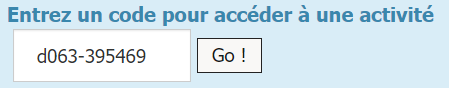
\includegraphics[scale=0.5]{td04_capcode}
	\end{center}
	\item laissez-vous guider sur le \cpy{notebook} et répondez aux différentes questions !
	\begin{center}
		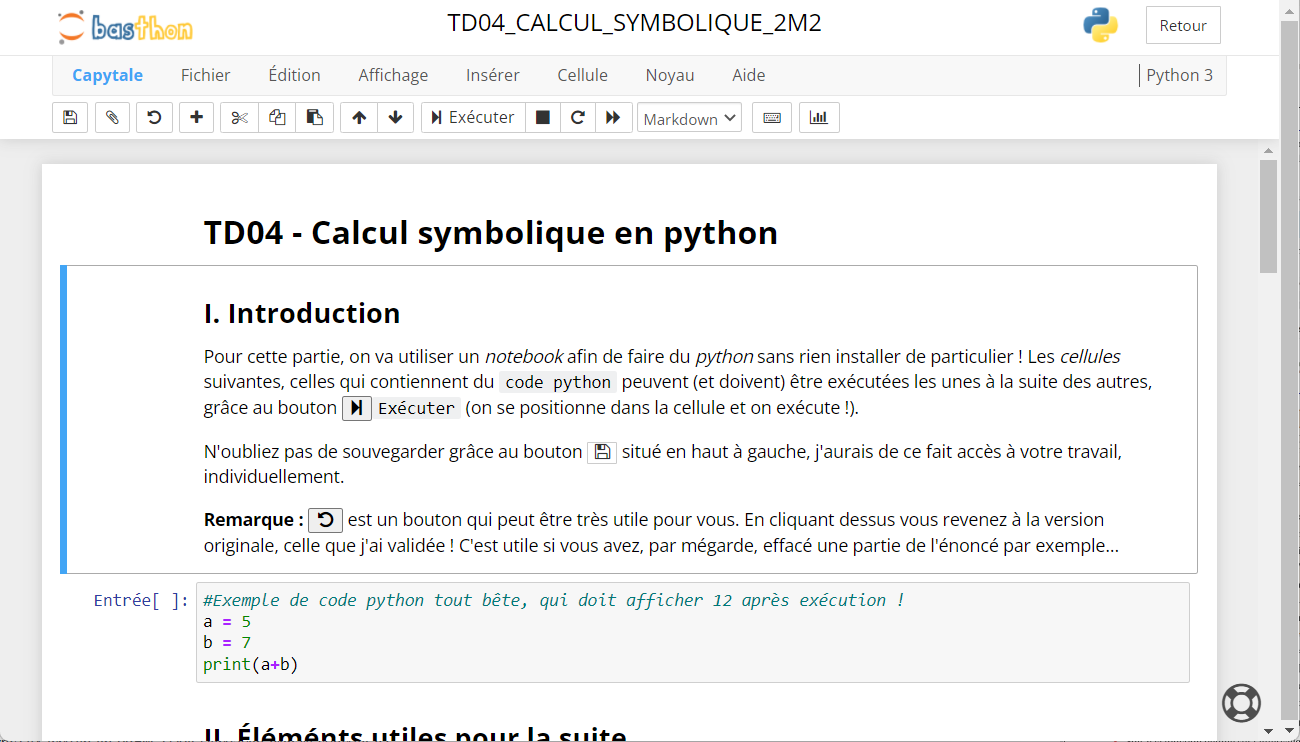
\includegraphics[scale=0.5]{td04_capcap}
	\end{center}
\end{itemize}

\medskip

\end{document}